\chapter{Chapter 4 : Routes and route matching}

\noindent This chapter is a guided tour of the route layer: how we build a unified view of routes from GTFS and HRDF, how the data looks, what the numbers show, and how we perform route-based matching between ATLAS stops and OSM nodes. Expect short code fragments, intuitive plots, and practical insights.

\section{From raw feeds to a single routes file}
\noindent This chapter expands on the overview introduced in Chapter~1; for clarity and flow, we repeat key ideas where helpful.
\subsection{What \texttt{atlas\_routes\_unified.csv} is}
We consolidate route evidence from two sources into a single tidy file:
\begin{itemize}
  \item \textbf{GTFS} (public transport feed): route identifiers, short/long names, and direction (0/1). Directions are derived using a \emph{first$\rightarrow$last} stop heuristic per trip, aggregated at route level.
  \item \textbf{HRDF} (railway schedule): line names and direction strings based on first$\rightarrow$last stations, both by name and by UIC code pairs.
\end{itemize}
Each row describes ``a route signal for a stop'':
\begin{center}
\small
\begin{tabular}{l l}
\toprule
Column & Meaning \\
\midrule
\texttt{sloid} & ATLAS stop identifier\\
\texttt{source} & \texttt{gtfs} or \texttt{hrdf}\\
\texttt{evidence} & Inference method (e.g. \texttt{gtfs\_first\_last}, \texttt{hrdf\_fplan})\\
\texttt{as\_of} & Date stamp for the evidence\\
\texttt{route\_id}, \texttt{route\_id\_normalized} & Raw and year-normalized GTFS ID\\
\texttt{route\_name\_short}, \texttt{route\_name\_long} & GTFS route names\\
\texttt{line\_name} & HRDF line (if any)\\
\texttt{direction\_id} & GTFS direction 0/1 (string)\\
\texttt{direction\_name}, \texttt{direction\_uic} & Human and UIC first$\rightarrow$last strings\\
\bottomrule
\end{tabular}
\end{center}
This schema is produced directly by the unified writer. Year-normalization removes seasonal suffixes like \texttt{-j24} so similar routes align across years:
\begin{verbatim}
# get_atlas_data.py (simplified)
re.sub(r'-j\d+', '-jXX', route_id)
\end{verbatim}

\subsection{How we generate it (high level)}
At a high level (see \texttt{get\_atlas\_data.py}):
\begin{enumerate}
  \item Load GTFS in a streaming fashion; keep only Swiss stops (IDs starting with \texttt{85}).
  \item First pass over \texttt{stop\_times}: collect for every \texttt{trip\_id} the first and last Swiss stops; join with \texttt{trips} and \texttt{routes} to obtain route IDs and names.
  \item Build per-route direction strings as ``first stop name $\rightarrow$ last stop name'' (deduplicated).
  \item Second pass over \texttt{stop\_times}: deduplicate \((\texttt{stop\_id},\ \texttt{route\_id},\ \texttt{direction\_id})\).
  \item Map GTFS \texttt{stop\_id} to ATLAS \texttt{sloid} (strict rule first, then safe fallbacks).
  \item Parse HRDF (\texttt{GLEISE\_LV95}, \texttt{FPLAN}, \texttt{BAHNHOF}) to get lines and first$\rightarrow$last directions per \texttt{sloid}.
  \item Write one tidy CSV combining both sources.
\end{enumerate}

\section{What the unified data says}
We computed the following from the existing unified file using scripts under \texttt{memoire/scripts\_used/chap4}. Outputs are archived in \texttt{memoire/data/processed/chap4/}.

\subsection*{GTFS view}
From \texttt{unified\_stats.json}:
\begin{itemize}
  \item \textbf{SLOIDs with GTFS routes}: \textbf{34,781}
  \item \textbf{Avg unique routes per \texttt{sloid}}: \textbf{2.73} (median \textbf{2.00})
  \item \textbf{Avg unique (route, direction) per \texttt{sloid}}: \textbf{4.39} (median \textbf{3.00})
  \item \textbf{Duplicate groups for (\texttt{sloid}, route\_norm, direction)}: \textbf{96.96\%}
  \item \textbf{Same route+dir, multiple direction strings}: \textbf{96.95\%} of such groups show more than one first$\rightarrow$last string (reflecting heterogeneous trip patterns)
\end{itemize}

\subsection*{HRDF view}
Also from \texttt{unified\_stats.json}:
\begin{itemize}
  \item \textbf{SLOIDs with HRDF lines}: \textbf{28,757}
  \item \textbf{Avg unique lines per \texttt{sloid}}: \textbf{2.32} (median \textbf{2.00})
  \item \textbf{Avg distinct directions per (\texttt{sloid}, line\_name)}: \textbf{2.67} by UIC and \textbf{2.67} by name (medians \textbf{2.00})
  \item \textbf{Long tails}: several (\texttt{sloid}, line) pairs show \textbf{30–40} distinct first$\rightarrow$last UIC pairs (heavy interlining/short-turns)
\end{itemize}

\section{A look at Geneva}
We plotted Geneva using only local files (no downloads): \texttt{data/raw/osm\_data.xml}, \texttt{data/processed/atlas\_routes\_unified.csv}, and \texttt{data/raw/stops\_ATLAS.csv}.

\begin{figure}[H]
  \centering
  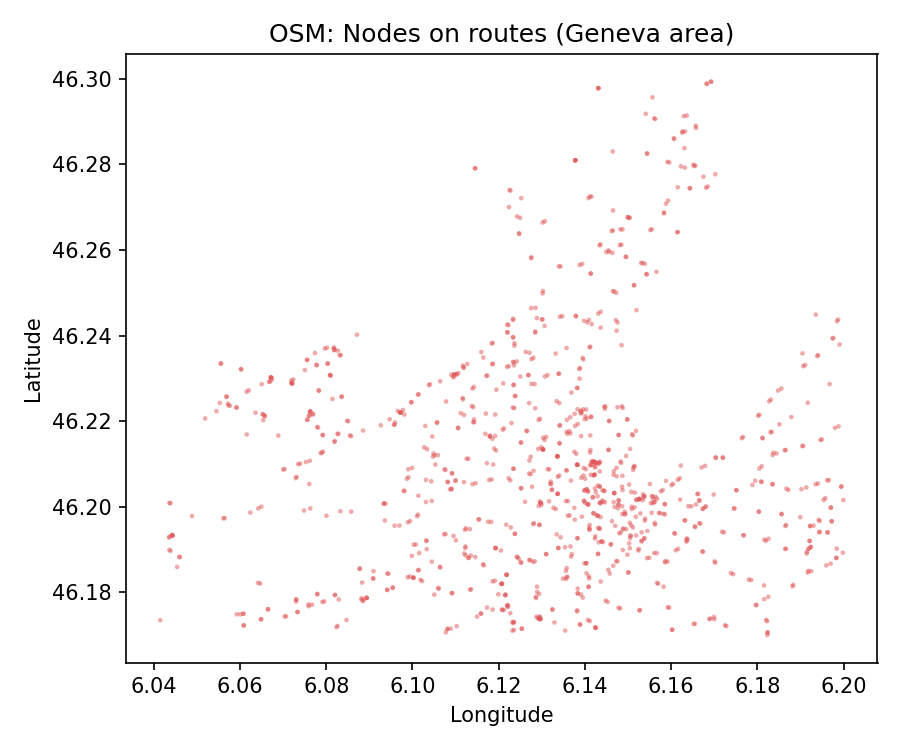
\includegraphics[width=0.8\textwidth]{../figures/chap4/geneva_osm_routes_nodes.png}
  \caption{OSM nodes that belong to at least one route relation (Geneva area).}
\end{figure}

\begin{figure}[H]
  \centering
  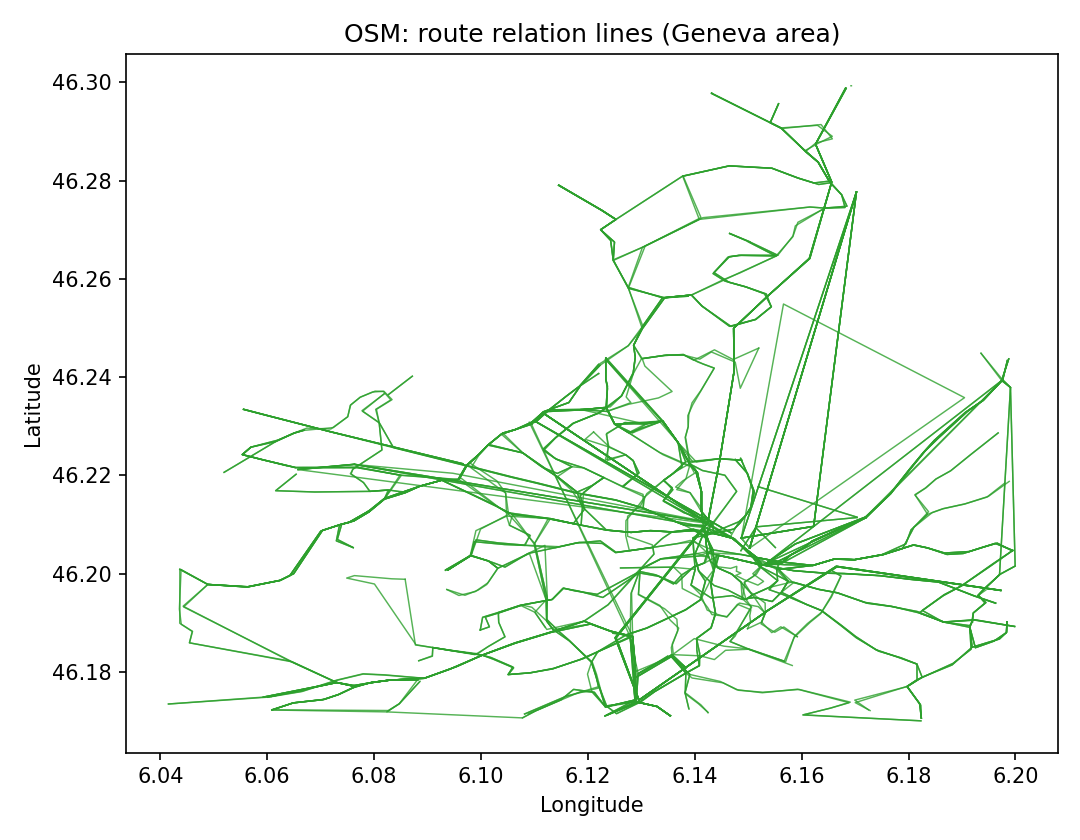
\includegraphics[width=0.8\textwidth]{../figures/chap4/geneva_osm_route_lines.png}
  \caption{OSM route layer: linework from route relations (Geneva). Well-structured geometry.}
\end{figure}

\begin{figure}[H]
  \centering
  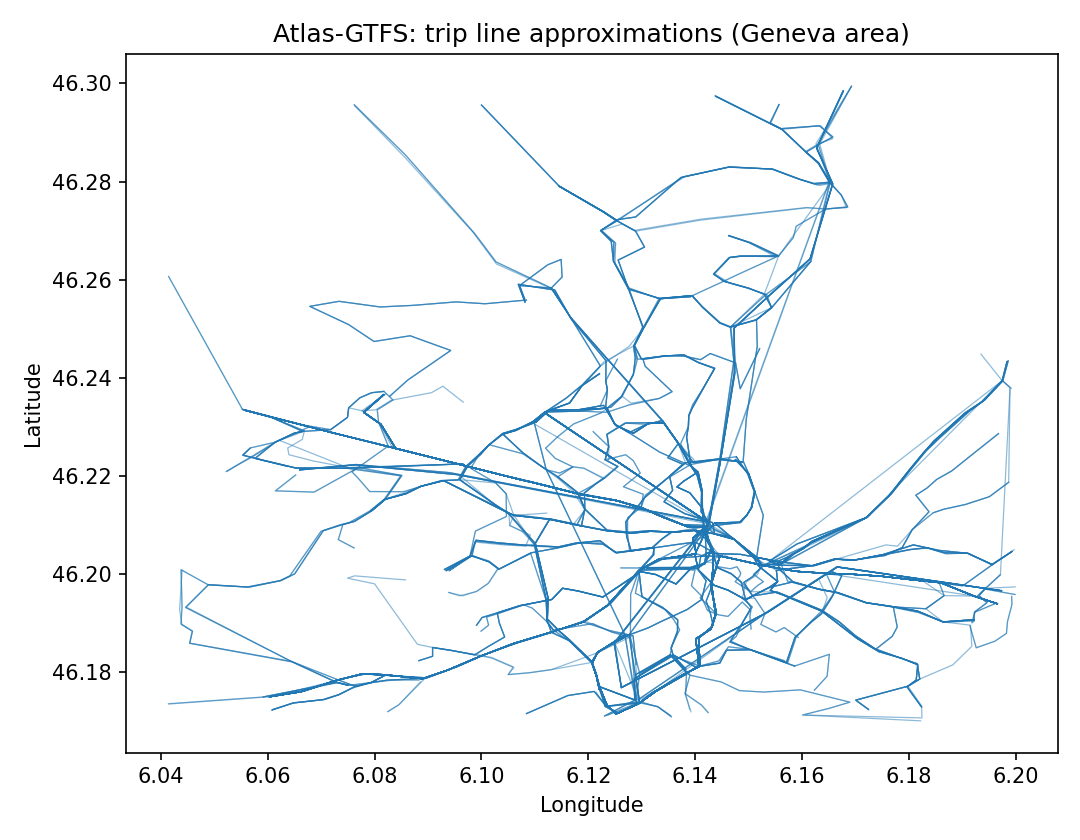
\includegraphics[width=0.8\textwidth]{../figures/chap4/geneva_gtfs_trip_lines.png}
  \caption{GTFS: trip-line approximations (Geneva). Lines reconstructed from stop order — more fragmented.}
\end{figure}

\begin{figure}[H]
  \centering
  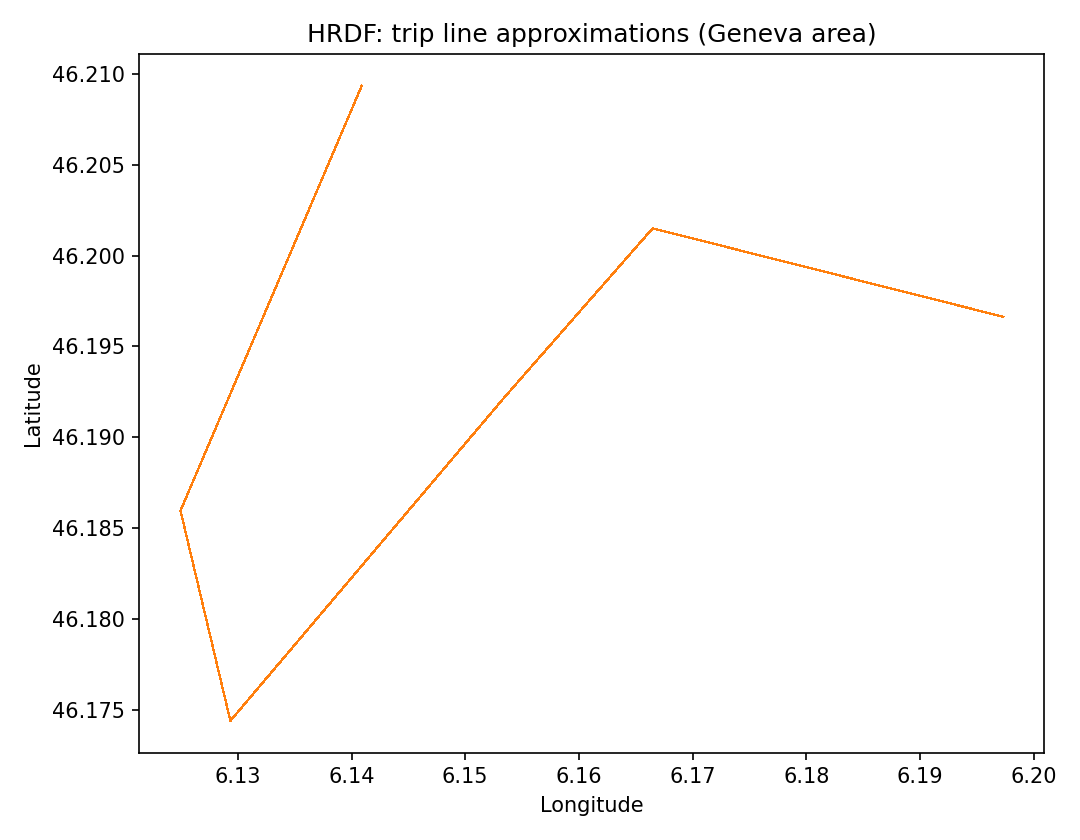
\includegraphics[width=0.8\textwidth]{../figures/chap4/geneva_hrdf_trip_lines.png}
  \caption{HRDF: trip-line approximations (Geneva). Derived from \texttt{FPLAN} sequences via UIC.}
\end{figure}

\section{More views worth having}
\begin{figure}[H]
  \centering
  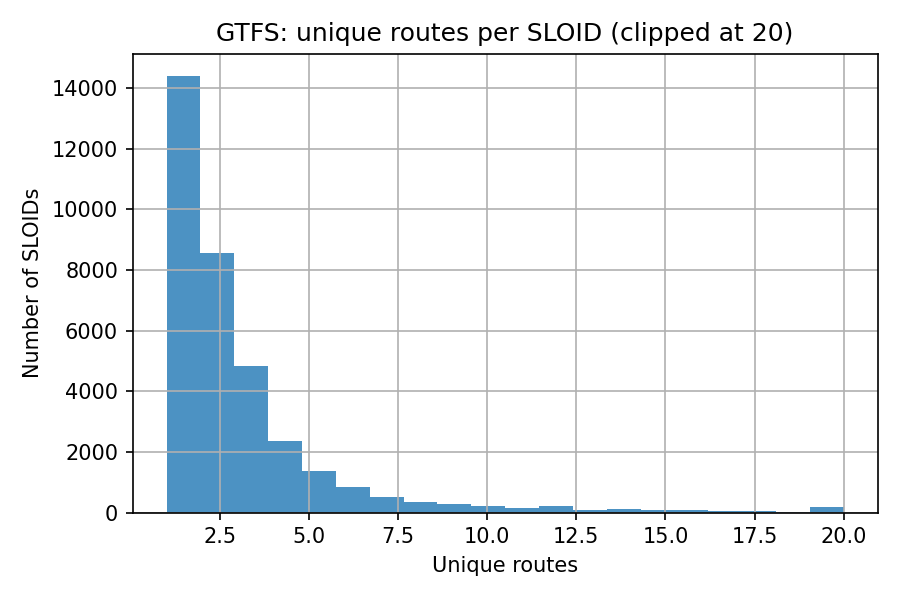
\includegraphics[width=0.75\textwidth]{../figures/chap4/hist_gtfs_routes_per_sloid.png}
  \caption{Distribution of unique GTFS routes per \texttt{sloid} (clipped at 20).}
\end{figure}

\begin{figure}[H]
  \centering
  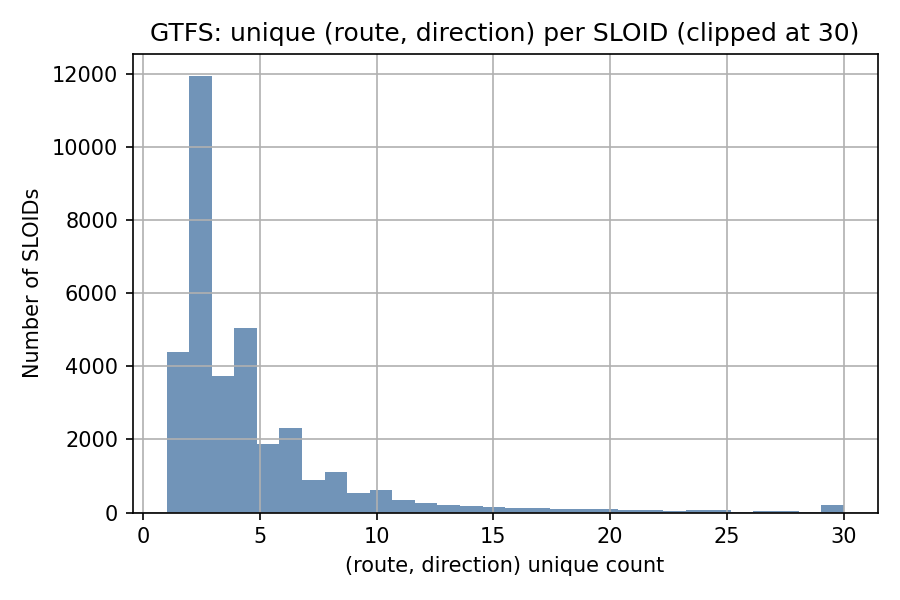
\includegraphics[width=0.75\textwidth]{../figures/chap4/hist_gtfs_route_dir_per_sloid.png}
  \caption{Distribution of unique (route, direction) per \texttt{sloid} (clipped at 30).}
\end{figure}

\begin{figure}[H]
  \centering
  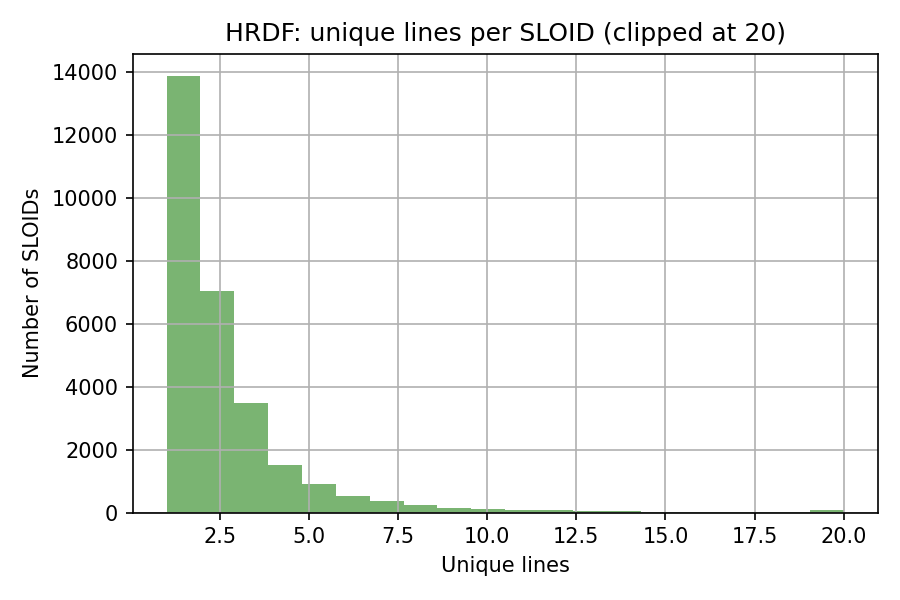
\includegraphics[width=0.75\textwidth]{../figures/chap4/hist_hrdf_lines_per_sloid.png}
  \caption{Distribution of unique HRDF lines per \texttt{sloid} (clipped at 20).}
\end{figure}

\subsection*{How we derive HRDF UIC direction tokens}
In Chapter~1 we outlined the HRDF parsing. Here we restate the essentials because these tokens are central to route matching:
\begin{itemize}
  \item From \texttt{GLEISE\_LV95}, we map each \texttt{sloid} to its station \texttt{UIC} and platform reference (\texttt{\#ref}).
  \item From \texttt{FPLAN}, for trips that touch those \((UIC,\ \#ref)\) pairs, we extract the first and last stops (UIC codes) and the line name (\texttt{*L}).
  \item Using \texttt{BAHNHOF}, we attach names to UICs and build both name-based and UIC-based direction strings: e.g., \texttt{"Genève $\rightarrow$ Lausanne"} and \texttt{"8501008 $\rightarrow$ 8501120"}.
\end{itemize}
These ``direction UIC'' tokens \((\texttt{line\_name},\ \texttt{direction\_uic})\) are then compared with OSM-derived first$\rightarrow$last UIC strings to support HRDF-level matching when GTFS identifiers are absent on OSM.

\section{Route matching: how it works}
The matching uses nearby OSM nodes and compares their route ``tokens'' against what we know for each ATLAS \texttt{sloid}. Tokens are either GTFS \((\texttt{route\_id},\ \texttt{direction\_id})\) (with optional year normalization) or HRDF \((\texttt{line\_name},\ \texttt{direction\_uic})\).

\subsection{Distance candidates}
We first collect nearby OSM nodes via a KD-tree within a configurable radius (default \texttt{50m}). Among these candidates we try matching in four tiers:
\begin{enumerate}
  \item \textbf{P1/P2 (GTFS tokens)}: any intersection between the \texttt{sloid}'s GTFS tokens and a candidate node's tokens.
  \item \textbf{P3 (HRDF by UIC)}: if an HRDF UIC first$\rightarrow$last string appears for that candidate's relation membership.
  \item \textbf{P4 (Names fallback)}: if a candidate has an OSM-derived first$\rightarrow$last \emph{name} string that matches any unified direction name for the \texttt{sloid}.
\end{enumerate}
Tiny excerpt of the token logic (simplified):
\begin{verbatim}
# For a candidate node, derive tokens from its routes
node_tokens = set()
for route in node_routes:
    rid = route.gtfs_route_id
    did = route.direction_id or '0'
    if rid:
        node_tokens.add((rid, did))
        rid_norm = normalize_route_id(rid)  # '-j25' -> '-jXX'
        if rid_norm:
            node_tokens.add((rid_norm, did))

# Check intersection with SLOID GTFS tokens
if gtfs_tokens & node_tokens:
    match = ('gtfs', 'gtfs_tokens')
\end{verbatim}

The route-id normalization used across the system is:
\begin{verbatim}
def normalize_route_id(route_id: str) -> str:
    return re.sub(r'-j\d+', '-jXX', route_id)
\end{verbatim}

\subsection{Configurations}
\begin{itemize}
  \item \textbf{Radius}: default \texttt{50m}. Smaller radii reduce false positives but may miss stops displaced in OSM.
  \item \textbf{Token types}: enable/disable GTFS-only tiers or include HRDF tiers.
  \item \textbf{Normalization}: route IDs can be normalized (\texttt{-jXX}) before comparison.
\end{itemize}

\section{Route matching: what the numbers say}
Using the optimized script (\texttt{route\_matching\_stats.py}, run on existing files), we obtain:
\begin{itemize}
  \item \textbf{GTFS tokens}: \texttt{7,252}; \textbf{OSM tokens}: \texttt{7,121}; \textbf{overlap}: \texttt{3,200}; \textbf{Jaccard}: \textbf{0.2864}
  \item \textbf{Per-\texttt{sloid} GTFS token coverage}: mean \textbf{2.64}, median \textbf{2}, p90 \textbf{6}; any coverage on \textbf{73.4\%} of \texttt{sloid}s
  \item \textbf{Route-level}: unique GTFS routes \textbf{3,839}; with an OSM match \textbf{1,664} $\rightarrow$ \textbf{43.3\%} route match rate
  \item \textbf{HRDF first$\rightarrow$last UIC strings}: HRDF \textbf{8,818}, OSM \textbf{5,633}, overlap \textbf{2,935}
\end{itemize}
Coverage as a histogram:
\begin{figure}[h]
  \centering
  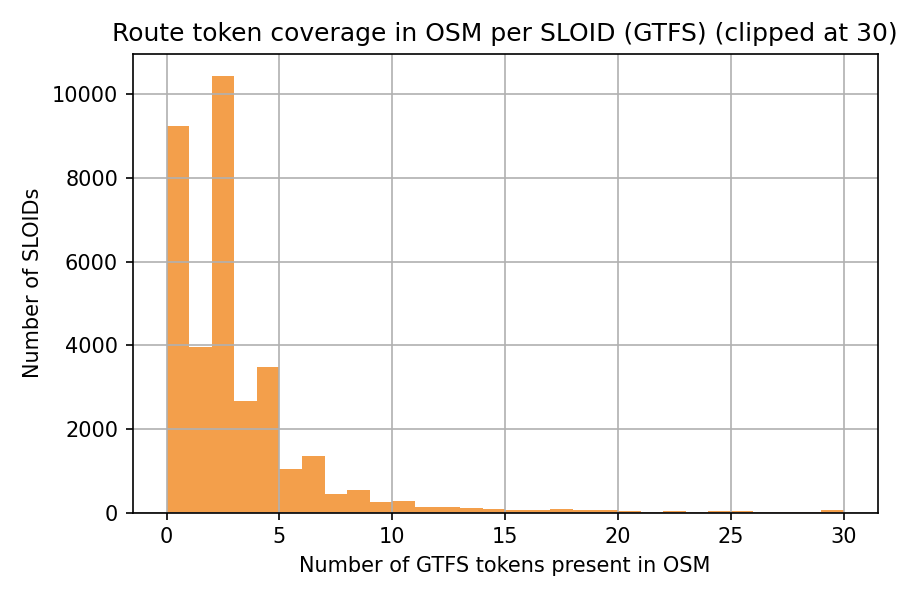
\includegraphics[width=0.75\textwidth]{../figures/chap4/hist_route_token_coverage_per_sloid.png}
  \caption{How many GTFS \((route, direction)\) tokens per \texttt{sloid} are found in OSM (clipped at 30).}
\end{figure}

\section{Scripts used for this chapter}
All scripts live under \texttt{memoire/scripts\_used/chap4} and operate only on files in \texttt{data/raw} and \texttt{data/processed}:
\begin{itemize}
  \item \texttt{compute\_unified\_stats.py}: reads \texttt{atlas\_routes\_unified.csv}, writes stats JSON/MD and histograms.
  \item \texttt{geneva\_maps.py}: produces the Geneva OSM/GTFS/HRDF plots.
  \item \texttt{route\_matching\_stats.py}: computes token overlaps and coverage summaries; optimized with progress logs and a fast mode.
\end{itemize}

\section{Reflection and next steps}
\textbf{Strengths}. The unified approach provides a compact, analyzable view of routes per stop across feeds. The matching pipeline favors precision (token intersections) backed by conservative distance thresholds. Year-normalization improves stability across timetable versions.

\textbf{Observed complexities}.
\begin{itemize}
  \item \emph{Multiplicity of directions}: Even for the same route+direction, many distinct first$\rightarrow$last strings exist, reflecting real operations (short turns, branches).
  \item \emph{Partial OSM tagging}: Many relations carry \texttt{gtfs:route\_id} but fewer expose robust direction cues; coverage is good but not complete.
  \item \emph{Spatial drift}: Small geocoding mismatches (or node placement) can push true candidates outside strict radii in dense hubs.
\end{itemize}

\textbf{Improvements}.
\begin{itemize}
  \item Incorporate sequence-level consistency: compare short path segments near the stop against GTFS stop order to disambiguate dense clusters.
  \item Learnable scoring: stack features (distance, tokens, name similarity, HRDF cues) into a trained ranker with human-labeled pairs.
  \item Direction robustness: distill many first$\rightarrow$last strings into a small set of canonical termini per route branch.
  \item Incremental refresh: cache token sets per feed version and re-match only impacted \texttt{sloid}s.
\end{itemize}

\noindent Bottom line: route-based matching adds a strong, independent signal that complements exact/name/distance methods. With a few targeted enhancements, coverage and confidence can both increase while keeping the pipeline fast and interpretable.
